% Created 2021-10-29 Fri 15:58
% Intended LaTeX compiler: pdflatex
\documentclass[11pt]{article}
\usepackage[utf8]{inputenc}
\usepackage[T1]{fontenc}
\usepackage{graphicx}
\usepackage{grffile}
\usepackage{longtable}
\usepackage{wrapfig}
\usepackage{rotating}
\usepackage[normalem]{ulem}
\usepackage{amsmath}
\usepackage{textcomp}
\usepackage{amssymb}
\usepackage{capt-of}
\usepackage{hyperref}
\author{Jonatan Ahumada}
\date{\today}
\title{To Be}
\hypersetup{
 pdfauthor={Jonatan Ahumada},
 pdftitle={To Be},
 pdfkeywords={},
 pdfsubject={},
 pdfcreator={Emacs 27.2 (Org mode 9.4.6)}, 
 pdflang={English}}
\begin{document}

\maketitle
\tableofcontents


\section{Identificación de problemas}
\label{sec:orgeff15b6}

\subsection{Nuevas tecnologías}
\label{sec:orgdc8bc20}

\begin{enumerate}
\item La trazabilidad del inventario se hace de forma manual y es propenso
a errores. Una posible solución es automatizar la solicitud del material,
el consiguiente descuento del inventario. El rol del almacenista solo sería
tomar la unidad en el almacén y prepararla para el confeccionista. El
resto podría automatizarse.

\end{enumerate}

\begin{enumerate}
\item El proceso de tiqueteo es fundamental para asegurar la calidad de la
prenda. Sin embargo, la creación de etiquetas se hace de forma manual,
cuando podría automatizarse. Las tendencias en confección textil
apuntan hacia el uso de escáneres 3D y 2D para nombrar y/o numerar
cada segmento de trazado sobre el textil ya trazado y extendido
sobre una superficie. El escaneo disminuirá la posibilidad del
error manual y además hará posible la posterior inspección automatizada
de la prende en el proceso de inspección de la confección.
\end{enumerate}


\subsection{Cambios en la operación}
\label{sec:org1d647b7}

\begin{enumerate}
\item La culminación del proceso de requisicón y compras era una notifiación
'manual' al confeccionista. Este luego buscaba manualmente el inventario,
como se ha descrito anteriormente. Sin embargo, una forma más optima de ver
el producto es lanzar una señal que recibirán tanto el almacenista
como el operario de transporte, para que inicien sus posteriores procesos.
\end{enumerate}



\subsection{Procesos To-Be}
\label{sec:orga70728b}

\begin{center}
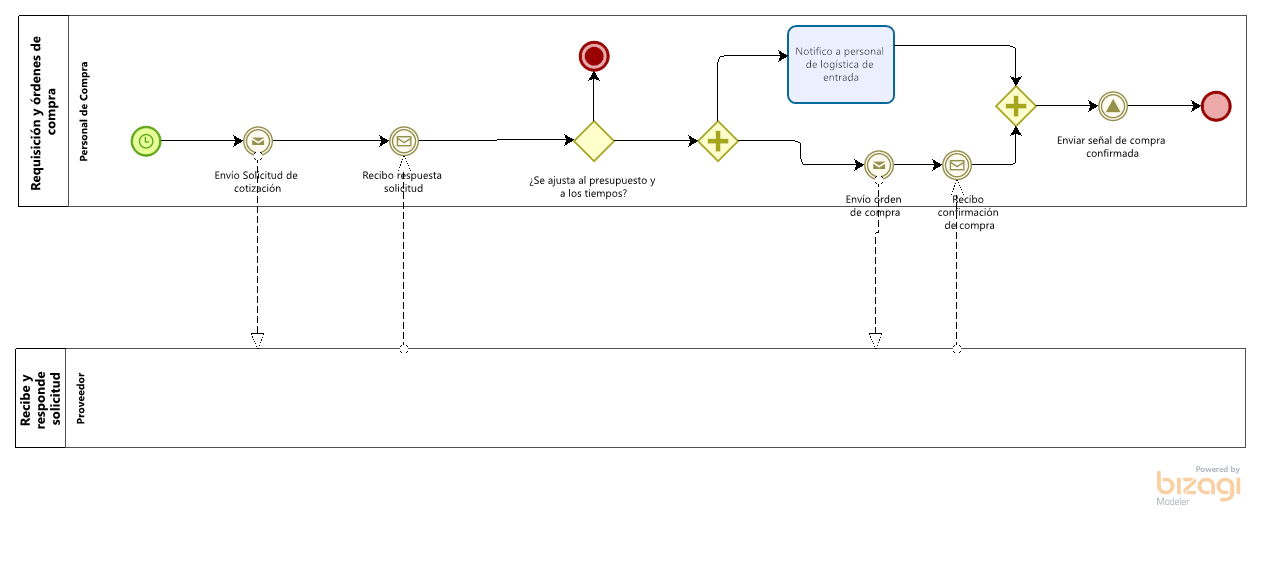
\includegraphics[width=.9\linewidth]{./assets/build/to_be/requisicion_compra.png}
\end{center}

\begin{center}
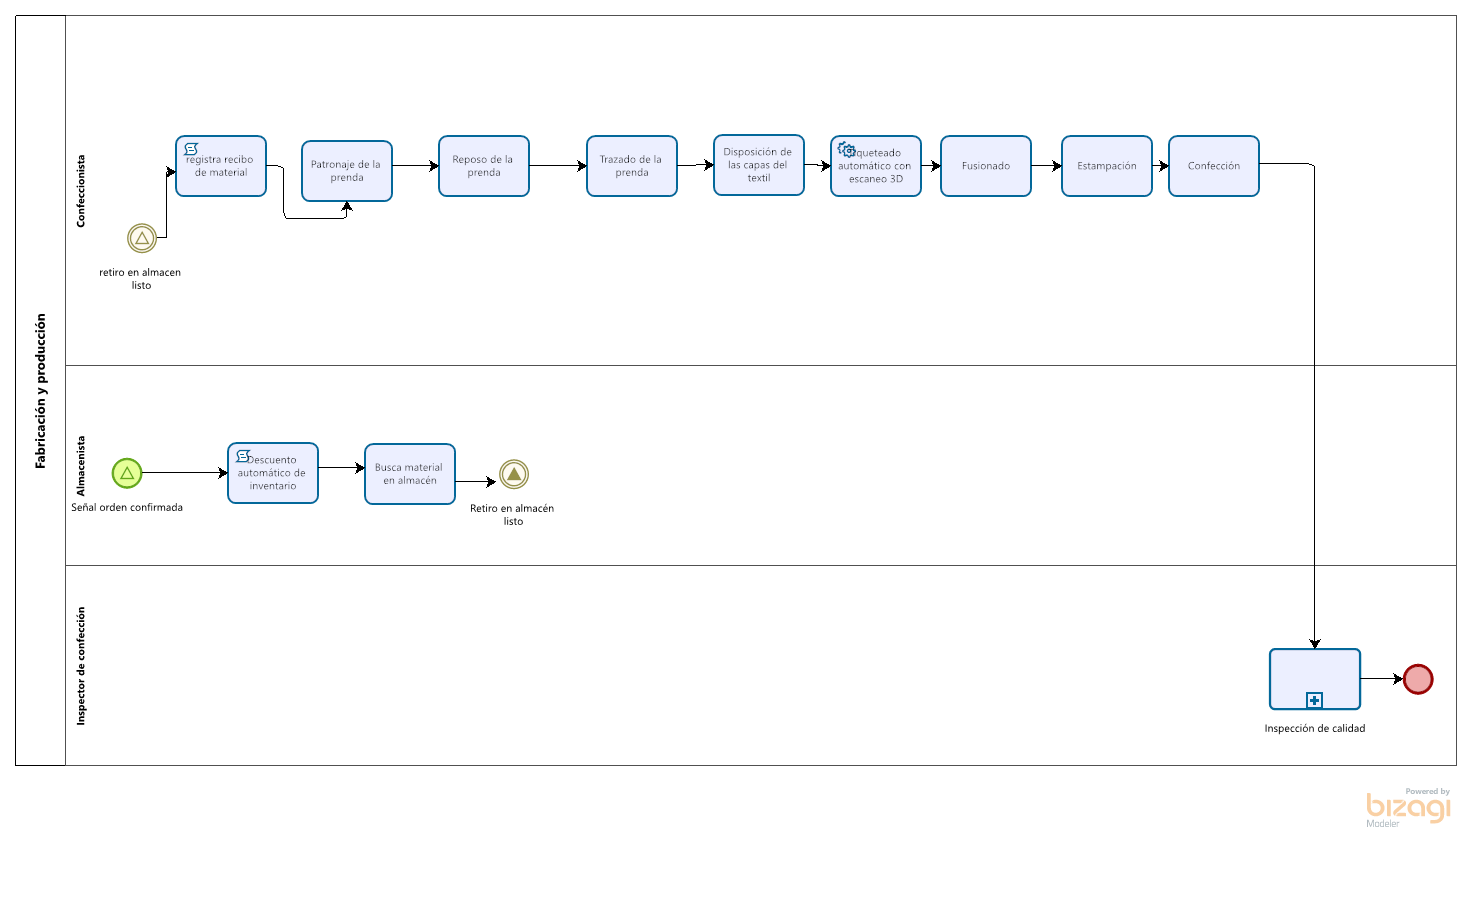
\includegraphics[width=.9\linewidth]{./assets/build/to_be/fabricacion_produccion.png}
\end{center}

\begin{center}
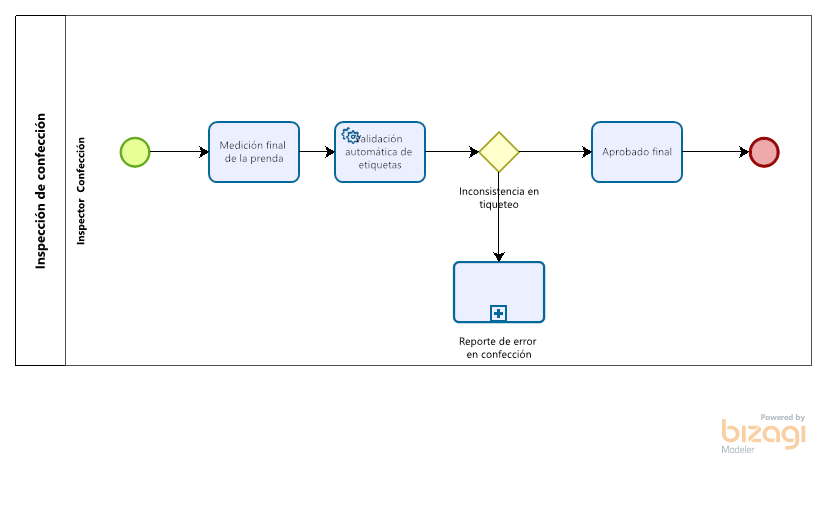
\includegraphics[width=.9\linewidth]{./assets/build/to_be/inspeccion_confeccion.png}
\end{center}

\begin{center}
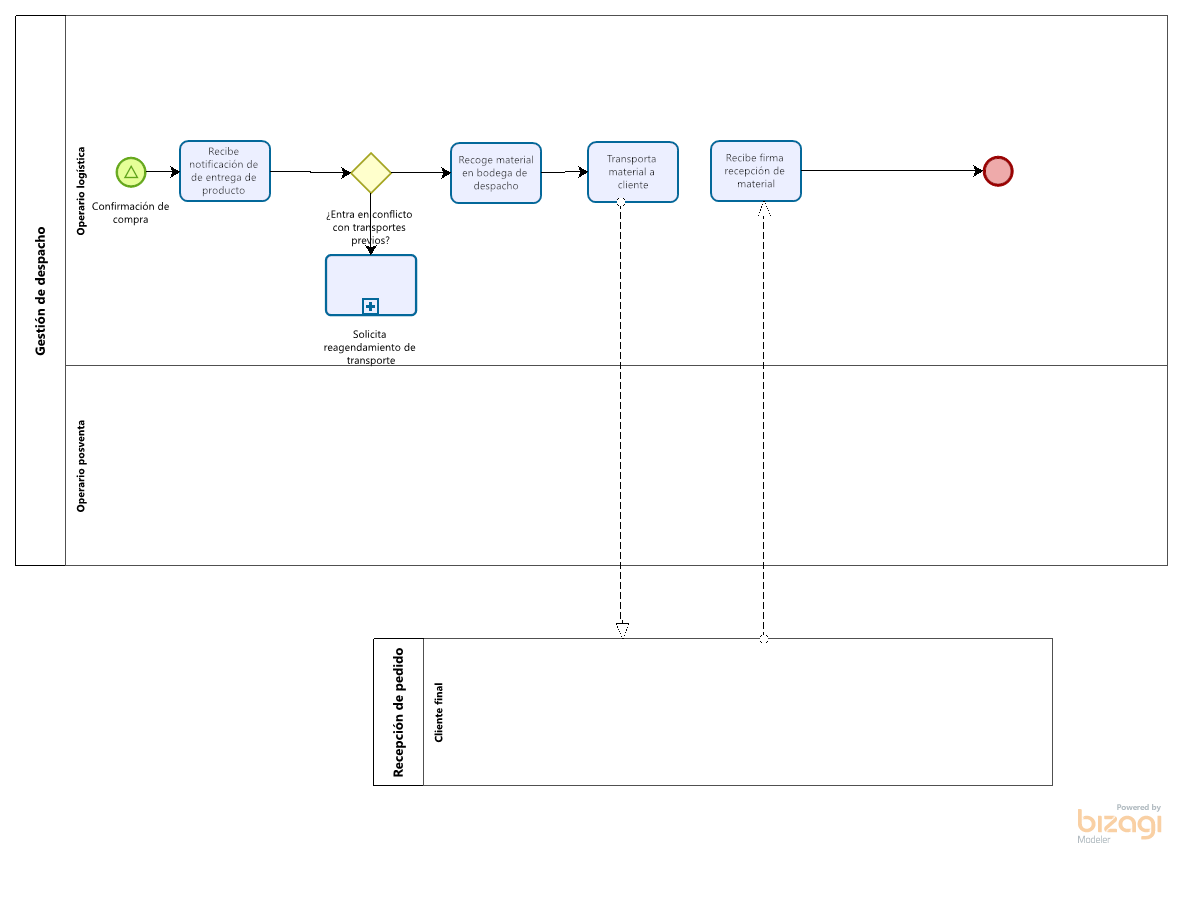
\includegraphics[width=.9\linewidth]{./assets/build/to_be/gestion_despacho.png}
\end{center}
\end{document}   Se identificó que en el proceso de Fabricación y producción las actividades
   que desarrolla el almacenista se hacen actualmente de forma manual.
   La trazabilidad del inventario se hace de forma manual y es propenso
   a errores. Una posible solución es automatizar la solicitud del material,
   el consiguiente descuento del inventario. El rol del almacenista solo sería
   tomar la unidad en el almacén y prepararla para el confeccionista. El
   resto podría automatizarse.
 
